% Limpa cabeçalhos.
% (solução para lidar com a númeração das páginas pré-textuais).
\pagestyle{empty}

%% Capa
\begin{titlepage}
	\begin{center}
		\textsc{\instituicao}
		\par
		\textsc{\eixo}
		\par
		\textsc{\curso}
		\par
		\vspace{130pt}
		\textsc{\autor}
		\vspace{130pt}
		\par
		\textbf{\Large{\titulo}}
		\par
		\vfill
		\textsc{\local}
		\par	
	      \ano
	\end{center}
\end{titlepage}

% Faz com que a página seguinte sempre seja ímpar (insere pg em branco)
\cleardoublepage

% Numeração em elementos pré-textuais é opcional (ativada por padrão).
% Para desativá-la comente a linha abaixo.
%\pagestyle{fancy}

% Números das páginas em algarismos romanos
\pagenumbering{roman}

%% Página de Rosto

% Numeração não deve aparecer na página de rosto.
\thispagestyle{empty}

\begin{center}
	\textsc{\autor}
	\par
	\vspace{200pt}
	\textbf{\Large \titulo}
\end{center}
	\par
	\vspace{90pt}
	
	%espaçamento simples
	\begin{singlespacing}
	
		\hspace*{175pt}\parbox{7.6cm}{\preambulo}
		
		\par
		\vspace{3em}
		\hspace*{175pt}\parbox{7.6cm}{Orientador: \orientador}
		\par
		\hspace*{175pt}\parbox{10cm}{Coorientador: \coorientador}

	\end{singlespacing}
	
	\par
	\vfill
\begin{center}
	\local
	\par
	\ano
\end{center}

\newpage

% Ficha Catalográfica

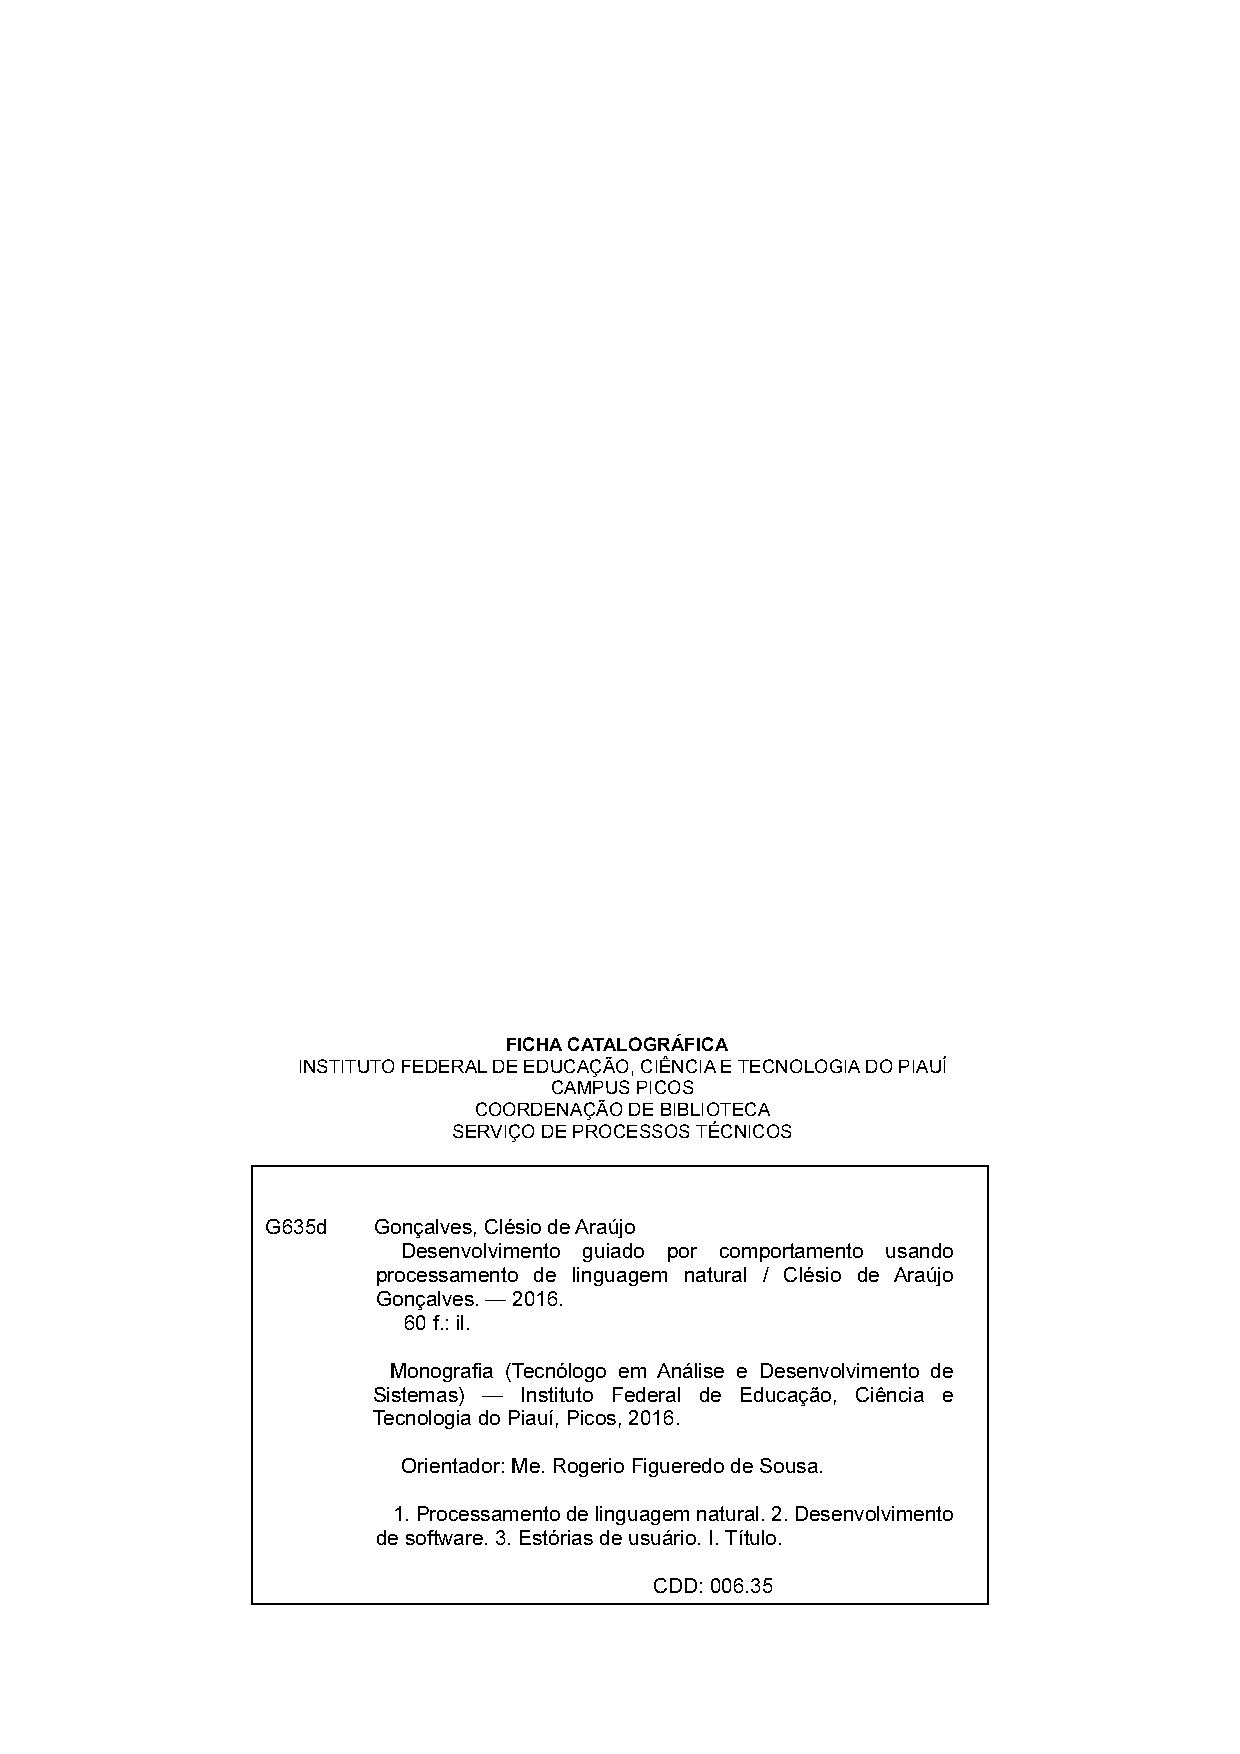
\includepdf[pages=1]{ficha/ficha_catalografica.pdf}

\newpage

%% Folha de Aprovação

% Numeração não deve aparecer na folha de aprovação.
\thispagestyle{empty}

\begin{center}
	\textsc{\autor}
	\par
	\vspace{60pt}
	\textbf{\Large \titulo}
\end{center}
\par
\vspace{60pt}

%espaçamento simples
\begin{singlespacing}

	\hspace*{175pt}\parbox{7.6cm}{\preambulo}

	\par
	\vspace{3em}
	Aprovado em \hspace{30pt}/\hspace{30pt}/     
	\vspace{3em}
	\begin{center}
		\textsc{\Large Banca Examinadora}

		\par
		\vspace{4em}
			%\extracolsep{\fill} = preenche a coluna
			\begin{tabular*}{\textwidth}{@{\extracolsep{\fill}}l l}
				\rule{18em}{1px} 				& \rule{18em}{1px} \\
				Prof. \orientador  				& Prof. \coorientador \\
				(Orientador)					& (Coorientador) \\
				Mestre em Ciência da Computação			& Especialista em Banco de Dados \\
				\instituto					& \instituto
			\end{tabular*}

		\par
		\vspace{4em}

		\parbox{22em}{\rule{22em}{1px} \\ %linha horiontal
		Prof. \convidado (Membro) \\
		Mestre em Engenharia de Produção \\
		\instituto} 
	\end{center}



	\par
	\vfill
	\begin{center}
		\local
		\par
		\ano
	\end{center}

\end{singlespacing}

\newpage

% Dedicatória
% Posição do texto na página
\vspace*{0.75\textheight}
\begin{flushright}
  \emph{Dedicatória...}
\end{flushright}

\newpage

% Agradecimentos

% Espaçamento duplo
%\doublespacing

\noindent{\LARGE\textbf{Agradecimentos}}

\vspace{2em}

Agradeço ao meu orientador, ao meu co-orientador, aos meus colaboradores, aos técnicos, à seção administrativa, à fundação que liberou verba para minhas pesquisas, aos meus amigos, à minha família e ao meu grande amor.

\newpage

% Epígrafe
\vspace*{0.3\textheight}
\noindent{\LARGE\textbf{Exemplo de epígrafe}}
% Tudo que você escreve no verbatim é renderizado literalmente (comandos não são interpretados e os espaços são respeitados)
\begin{verbatim}
O que é bonito?
É o que persegue o infinito;
Mas eu não sou
Eu não sou, não…
Eu gosto é do inacabado,
O imperfeito, o estragado, o que dançou
O que dançou…
Eu quero mais erosão
Menos granito.
Namorar o zero e o não,
Escrever tudo o que desprezo
E desprezar tudo o que acredito.
Eu não quero a gravação, não,
Eu quero o grito.
Que a gente vai, a gente vai
E fica a obra,
Mas eu persigo o que faltaoneside
Não o que sobra.
Eu quero tudo que dá e passa.
Quero tudo que se despe,
Se despede, e despedaça.
O que é bonito…
\end{verbatim}
\begin{flushright}
Lenine e Bráulio Tavares
\end{flushright}

\newpage

\vspace*{10pt}
% Abstract
\begin{center}
  \emph{\begin{large}Resumo\end{large}}\label{resumo}
\vspace{2pt}
\end{center}
% Pode parecer estranho, mas colocar uma frase por linha ajuda a organizar e reescrever o texto quando necessário.
% Além disso, ajuda se você estiver comparando versões diferentes do mesmo texto.
% Para separar parágrafos utilize uma linha em branco.
\noindent
Esta, quem sabe, é a parte mais importante do seu trabalho.
É o que a maioria das pessoas vai ler (além do título).
Seja objetivo sem perder conteúdo.
Um bom resumo explica porquê este trabalho é interessante, relata como foi feito, o que foi encontrado, contextualiza os resultados e delineia conclusões.
\par
\vspace{1em}
\noindent\textbf{Palavras-chave:} palavra1, palavra2, palavra3
\newpage

% Criei a página do abstract na mão, por isso tem bem mais comandos do que o resumo acima, apesar de serem idênticas.
\vspace*{10pt}
% Abstract
\begin{center}
  \emph{\begin{large}Abstract\end{large}}\label{abstract}
\vspace{2pt}
\end{center}

% Selecionar a linguagem acerta os padrões de hifenação diferentes entre inglês e português.
\selectlanguage{english}
\noindent
This is the most important part of your work.
This is what most people will read.
Be concise without omitting content.
A good abstract explains why this is an interesting study, tells how it was done, what was found, contextualizes the results and set conclusions.
\par
\vspace{1em}
\noindent\textbf{Keywords:} word1, word2, word3

% Voltando ao português...
\selectlanguage{brazilian}

\newpage

% Desabilitar protrusão para listas e índice
\microtypesetup{protrusion=false}

% Lista de figuras
\listoffigures

% Lista de tabelas
\listoftables

% Abreviações
% Para imprimir as abreviações siga as instruções em 
% http://code.google.com/p/mestre-em-latex/wiki/ListaDeAbreviaturas
\printnomenclature

% Índice
\tableofcontents

% Re-habilita protrusão novamente
\microtypesetup{protrusion=true}
